The last category of approaches to solve TSP are \emph{Metaheuristics} we're
going to present, high-level and complex procedures that are powerful enough to
reach near-optimum solutions in a reasonable amount of time, even with huge
instances. Considering the NP-hardness of TSP, this is our best shot so far, if
we're satisfied with an approximate solution. Internally they uses the
precedent heuristics we presented: they're placed at the implementation level
considering the high-level formulation of metaheuristics.\\ Among all the
approaches presented during the years, we're going to introduce three of them that
works nicely on TSP.

\section{Variable Neighborhood Search}
\emph{Variable Neighborhood Search} (VNS) is a metaheuristic technique proposed in
1997 \citep{mladenovic1997variable}. When an algorithm explores a solution space
not using mathematical programming the final result may be very influenced by
the starting solution. Sometimes allowing the algorithm only to improve the
solution can stuck it in local minimum that can be way worse than the optimal
solution. So VNS consents the current solution to move in a random way to
give it a chance to escape from these points of minimum.\\

\begin{algorithm}[H]
\SetAlgoLined
\KwResult{An approximated solution}
    $x\ \leftarrow$ initial solution\;
    \While{time limit is not reached \emph{or} $k \le k_{max}$}{
        $x'\ \leftarrow\ shake(x, k)$\;
	    $x' \leftarrow\ localopt(x')$\;
        \eIf{$cost(x') \le cost(x)$}{$x \leftarrow x'$\;}{$k \leftarrow k+1$\;}
    }
    \caption{VNS}
\end{algorithm}

So, the procedure of VNS needs two fundamental element: the method that
improves the solution and the one that can disturb it to escape from possible
local minimum. The \emph{shaking} function that disturbs the solution usually
depends on a input value $k$ that defines the neighborhood size Then the local
search function finds a local minimum. If this new solution is better then the
one before it becomes the incumbent, otherwise the neighborhood size increases
by one. If the max neighborhood size is reached the algorithm stops.

\subsubsection{Implementation details}
In our implementation of VNS we adapt the possibility to start from a random
solution or from a precomputed one. More on this choice in the next section,
since we're going to face similar choices. In TSP terms the shake operation is
called \emph{kick}, as it is slightly modifies the incumbent by rearranging $k$
arcs. The procedure clearly has to modify the solution into a feasible on, the
implemented procedure has to be subtour-free. The new candidate solution is then
modified using $2$-opt moves refinement presented is the previous chapter since,
as claimed, for an interesting number of nodes, there's no point of using
$k$-opt moves, with $k \ge 3$.\\ 
Every time a better solution is found the incumbent is updated and VNS is reset
with starting $k$ value equals to some minimum, 3 in our implementation. In the
case that the local search did not produce a new optimum the neighborhood is
enlarged by increasing $k$, until $k$ reaches $k_{max}$, where the algorithms
terminates. The increment of $k$ as well as $k_{max}$ should be tuned according
to the time limit, since it's not optimal to waste time on small $k$ with no
improvements or waste possibilities by truncating the computation due to small
$k_{max}$.\\
This can be seen as a multi-start procedure as the one presented above, but with
a kicked solution instead of a total different one.


\section{Tabu Search}
\emph{Tabu Search}, among with VNS, is another important metaheuristic proposed
by Fred Glover in 1986\citep{glover1986future} and, as VNS, is based on
refinements.\\ Starting from a solution, one is willing to improve it with
refinements until a local optimum is reached (\emph{downhill}). From there, one
could restart from another initial solution (multi-start) or restart from a
similar one by shaking it. Instead of those solutions, it's possible to insist
on the refinement subroutine and apply the refinement anyway. Since the solution
is stuck in a local optimum, the refinement will not improve the solution (it's
not a refinement at all!) but it will worse it. The idea is to apply as many
worsening move as possible until our subroutine produces a refinement that will
improve the solution (\emph{climbing}). At the end of this procedure, the
solution will be slightly different from the one stuck in the local optimum,
allowing us to restart from it in the refinement process.\\ To do so, an
important consideration has to be made: after the application of a worsening
move, the refinement subroutine will return a better solution by simply reverse
the move just done. For this reason, in the climbing part, it's important to
mark those moves as \emph{tabu}, forbidden moves that the refinement subroutine
will have to skip to produce a different starting solution.\\

\begin{algorithm}[H]
\SetAlgoLined
\KwResult{An approximated solution}
    $x\ \leftarrow$ initial solution\;
    \While{time limit is not reached}{
        $m\ \leftarrow\ move(x)$\;
        \If{$m$ is not tabu}{
            \If{$m$ is worsening move}{
                add $m$ to \emph{tabu list}
            }
            $x'\ \leftarrow\ apply\_move(x, m)$\;
        }
    }
    \caption{Tabu Search}
\end{algorithm}

Applied to TSP case, the refinement subroutine is $2$-opt move and the move is
the rearranging of 2 arcs. Initially, we will apply as many moves as possible in
order to improve the solution (\emph{downhill}). We can notice those moves by the
analysis of the $\Delta$ returned by the procedure: if $\Delta < 0$, it's an
improving move, otherwise it's a worsening one. After being stuck in a local
optimum, we can apply moves with $\Delta > 0$ until an improving one can be
found (\emph{climbing}) while marking all the nodes involved in the moves as
\emph{tabu nodes}. This is a simplification since we should declare the arcs
tabu (caused they're better representative of the move). Those nodes will be
stored in a \emph{tabu list} available to the $2$-opt move algorithm in order to
avoid them. We missed an important detail while defining the tabu moves: after
many iterations, almost every nodes will be marked as tabu. For that reason, we
have to release those nodes after some time, usually fixed, called
\emph{tenure}, which defines the maximum size of the tabu list. 

\subsubsection{Implementation details}
An initial solution has to be selected and, as in VNS, one could simply take it
randomly. A huge problem arise, because the first downhill could occupy the
majority of the time limit. $2$-opt moves are certain fast but still costly. To
explain this, let's analyze how $\Delta$ changes during iterations.

\begin{figure}[h!]
    \centering
    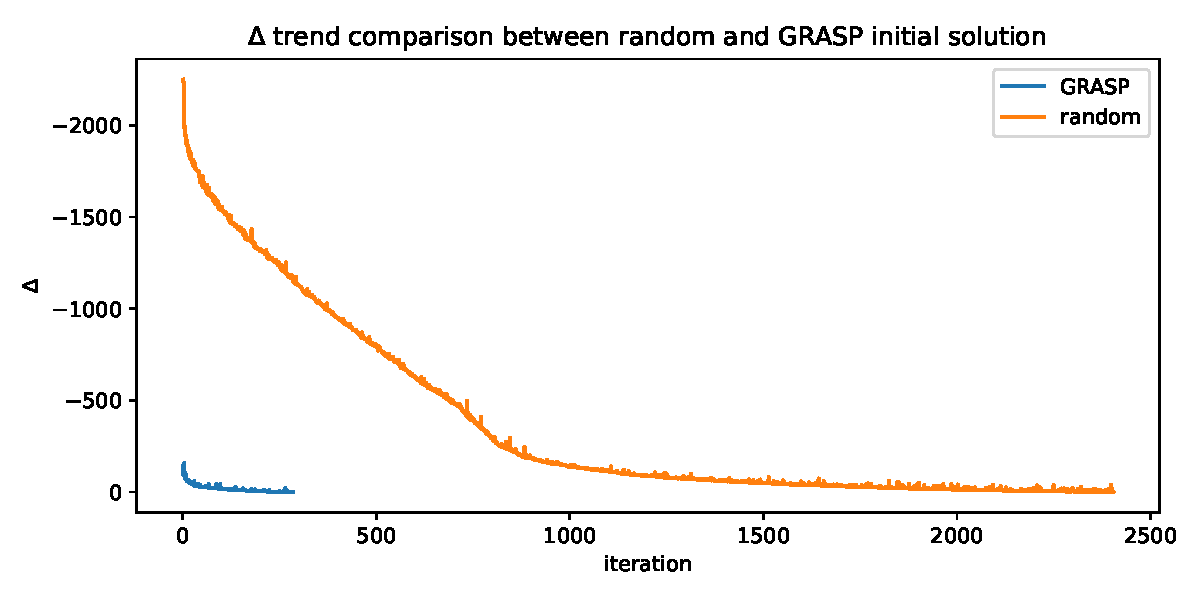
\includegraphics[width=0.78\textwidth]{figures/delta_trend}
    \caption{$\Delta$ trend for different initial solution.}
\end{figure}

This represent the typical trend of $\Delta$ for an instance centered in a 1000
x 1000 box (that explain $\Delta$ in absolute values) for the first downhill.
Future downhills and climbings are similar in the sense that both of them
occupies just few iterations each. Using a GRASP as feeder for an initial
solution (blue line), it's rare to encounter costly crossing (initials are
typically $\sim-100$) and $\Delta$ drops very quickly ($\Delta < 1$ in $\sim250$
iterations). For a random start the situation is different (orange line):
initial $\Delta$ could be very high and there's a typical linear drop followed
by a logaritmic one until no more moves are possible. This typically takes 10
times the iterations using GRAPS as initial solution. For that reason, we will
feed the algorithms using the best GRASP solution among 500 starts, so more time
will be spent on the object in analysis: metaheuristics.\\ One could reply by
saing that our future analysis will be bias against GRASP-ish solutions. Well,
we can't really argue against that, only partially. One could assert that among
the near-optimal solutions, GRAPS don't produces the best ones, even if refined.
We have to remind that refinement could change lot of tour structure and, in
general, don't produce the optimal one, just a very good one. So there is no way
to think that a initially random-refined solution will be better than a
GRAPS-refined one. This justifies the choice of GRAPS among all the constructive
heuristics presentend when dealing this kind of situations.\\ 
Another possible degree of freedom in Tabu Search implementation lies in the
tabu list. We keep the things as simple as possible, by tracking the iteration
number when the nodes were marked as tabu and compare it with the actual one: if
the difference is less than the tenure, the nodes is still tabu. There's no need
to implement an actual list, just an array of time stamps.\\
The last point is how to deal the neighborhood size while searching for
solutions. In this case the tenure play the same role as the kick strenght in
VNS: by letting it change it's possible to define two phases:
\emph{intesification} and \emph{diversification}. In the first one the tenure is
kept high and lots of nodes will be marked as tabu: there's a small degree of
freedom and new solution will be very similar to the actual one. In the second
one, in which the tenure is small, few nodes will be blocked and there's the
possibility to find very different solutions. A switch between this two phases
is beneficial. The tenure values as well as the phases length are chosen
according to the number of nodes for the first one and according to the time
limit for the second one: we let switch between the phases around two/three
dozen of times during computation.

\section{Genetic algorithm}
The genetic algorithm is one of the most popular metaheuristic techniques. It is
widely used in operation research and optimization problem and it inspired by
the natural selection. The idea behind the algorithm exploit the possibility to
merge two different elements of a population to create a new one that hopefully
combines the best characteristic of both parents generating a better element.
For this purpose, when a problem is defined, it is necessary to establish a
measure of performance that in our case is intrinsic considering we are dealing
with an optimization problem. 

\newpage
The process usually follows the same steps. First of all, a population of n
candidate solutions to the problem is generated with a significant randomness
component since diversity is a fundamental feature. Then, a percentage of these
candidates is paired and returns a new child solution from each pair combining
their chromosome, a data structure containing main information of the solution.
These children are inserted in the population and now among all the candidate
solutions the best n are kept alive. Iteration after iteration the population
will become better and better in terms of average quality. After a sufficient
number of iterations the hope is that new children will become the best
solutions resulting in a better near-optimum.

\begin{algorithm}[H]
\SetAlgoLined
\KwResult{An approximated solution}
    \emph{population} $\leftarrow$ n random solutions\;
    \While{last iteration i is reached}{
        sample 2k \emph{parent} solution from \emph{population}\;
        \ForEach{pair p} {
            \emph{population} $\leftarrow$ add p \emph{child}\;
        }
        \emph{population} $\leftarrow$ keep best n candidates\;
    }
    \emph{sol} $\leftarrow$ best candidate in \emph{population}
    \caption{Genetic Algorithm}
\end{algorithm}

\subsubsection{Implementation details}
In genetic algorithms implementation choices are mostly based on how solutions
are randomly generated, how they are map into a chromosome and how chromosomes
are combined. In case of TSP the most straightforward way to represent a
solution is an array of length n-nodes representing the order in which nodes are
visited. Those instances are created as a permutation of the first n-nodes
number taking the sequence from 1 to n-nodes and applying randomly $2$n-nodes
permutation. To combine two chromosome they are both split in left and right
part. Child left part is the same of parent 1. Then, all the nodes of parent 2
right part not visited by the child are added. In this way the child could not
visit all the nodes if a node $n_i$ is in parent 1 right part and parent 2 left
one. So the child generation performs extra-mileage to complete the solution. 

This procedure could be enough to implement a genetic algorithm but it turned
out to be inefficient because it led to a solution quite far from the optimum. A
valid way to find a solution closer to the best one can be obtained by adding a
2-opt refinement to both parents and children generation. It could seem a bit
against the spirit of the nature based idea but it really helps to converge to a
population of good solutions. Anyway with large instances it represent a major
burden and allows a very few number of iteration to combine the random
instances. After some tries with the algorithm we basically made a choice on the
number of nodes to decide whether or not to use any refinement. This decision
influence also the size of the population that can be handle. For small
instances it was possible to perform a 2-opt to both starting and children
instances, while for medium size TSP (around 500) only for children generation
and decreasing the population size. For very large instances the usage of these
refinement is not feasible at every iteration so the search among the population
is done in the most raw way and only when the final solution is chosen it is
refined.



